\documentclass[12pt]{report}
\setlength{\textwidth}{6.5 in}
\setlength{\evensidemargin}{0 in}
\setlength{\oddsidemargin}{0 in}
\setlength{\textheight}{9.4 in }
\setlength{\topmargin}{-0.7 in}
\pagestyle{myheadings}
\markboth{\em EE264: Homework \#02}{\em EE264: Homework \#02}
\usepackage[pdftex]{graphicx} \usepackage{eso-pic}
\usepackage{amsmath}
\usepackage{amssymb}
\usepackage{graphicx}
\usepackage{ifthen}
\usepackage{tikz}
\usepackage{pgfplots}
\usepackage{array}  % for table column M
\usepackage{makecell} % to break line within a cell
\usepackage{verbatim}
\usepackage{epstopdf}
\usepackage{amsfonts}
\usepackage{xcolor}
\usepackage{subcaption}
\usepackage{pdfpages}
%\captionsetup{compatibility=false}
%\usepackage{dsfont}
\usepackage[absolute,overlay]{textpos}
\usetikzlibrary{calc}
\usetikzlibrary{pgfplots.fillbetween, backgrounds}
\usetikzlibrary{positioning}
\usetikzlibrary{arrows}
\usetikzlibrary{pgfplots.groupplots}
\usetikzlibrary{arrows.meta}
\usetikzlibrary{plotmarks}

\DeclareGraphicsExtensions{.pdf,.eps,.png}

\DeclareMathOperator{\E}{\mathbb{E}} % expectation

\begin{document}
\thispagestyle{empty}
\begin{centering}
	{\large Stanford University}\\
	{\large EE 264: Digital Signal Processing}\\
	{\large Summer, 2017} \\
	\mbox{}\\
	{\large Homework \#02}\\
	\mbox{}\\
\end{centering}
\noindent Date assigned:  July 6, 2017 \hfill
Date due: July 13, 2017\\
\noindent \rule{6.5 in}{0.5pt}
%\mbox{}\\
\noindent {\bf Reading:}  This assignment covers lecture 3, which corresponds to the sections 4.1--4.9 of the text book {\bf DTSP 3e}. \\
\noindent {\bf Homework submission:}  Please submit your solutions on Canvas. Create a single .pdf file containing all your analytical derivations, sketches, plots, and Matlab code (if applicable). \\
\noindent {\bf Extra practice:}  Problems for extra practice are provided at the end of this assignment. Do \underline{not} turn in solutions to extra practice problems.

\noindent
\rule{6.5 in}{0.5pt}
\mbox{}\\

\noindent {\bf Problem 1: (25 points)}

Consider the generic discrete-time system discussed in class:

\begin{figure}[!h]
	\centering
	\resizebox{0.9\textwidth}{!}{\def\layersep{2cm}
\def\outsep{0.7cm}
\def\dy{1.25}

\begin{tikzpicture}[->, >=stealth, shorten >= 0pt, draw=black!50, node distance=\layersep, font=\sffamily]
    \tikzstyle{node}=[circle,fill=black,minimum size=2pt,inner sep=0pt]
    \tikzstyle{block}=[draw=black,rectangle,fill=none,minimum size=1.5cm, inner sep=0pt]
    \tikzstyle{annot} = []

	\node[node] (xc) at (0, -\dy cm) {};
    \node[block] (ADC) at (1*\layersep, -\dy cm) {C-to-D};
    \node[block, text width = 2cm, align= center] (DSP) at (3*\layersep, -\dy cm) {LTI \\ System};
    \node[block] (DAC) at (5*\layersep, -\dy cm) {D-to-C};
	\coordinate (yc) at (6*\layersep, -\dy cm) {};
	
	\coordinate (mid1) at ($(ADC.east)!0.5!(DSP.west)$) {};
	\coordinate (mid2) at ($(DSP.east)!0.5!(DAC.west)$) {};
		
    \path (xc) edge (ADC);
    \path (ADC) edge (DSP);
    \path (DSP) edge (DAC);
    \path (DAC) edge (yc);
    
    \node[above = 0.5mm of mid1] {$x[n]$};
    \node[below = 0.5mm of mid1] {$X(e^{j\omega})$};
    \node[above = 0.5mm of mid2] {$y[n]$};
    \node[below = 0.5mm of mid2] {$Y(e^{j\omega})$};
    \node[above = 0mm of xc, text width = 1cm, align=center] {$x_c(t)$};
    \node[below = 0mm of xc, text width = 1cm, align=center] {$X_c(j\Omega)$};
    \node[above = 0mm of yc, text width = 1cm, align=center] {$y_r(t)$}; 
    \node[below = 0mm of yc, text width = 1cm, align=center] {$Y_r(j\Omega)$};
    \node at ($(DSP.south)-(0, 0.25cm)$) {$h[n] \leftrightarrow H(e^{j\omega})$};
\end{tikzpicture}}
	\caption{Diagram for discrete-time processing of continuous-time signals.}
\end{figure}

Let's assume that input signal $x_c(t)$ and the discrete-time LTI system $h[n]$ have the following frequency-domain representation:

\begin{figure}[h]
	\begin{subfigure}[t]{0.5\textwidth}
		\centering
		\resizebox{\textwidth}{!}{\begin{tikzpicture} 
\begin{axis}[
axis lines*=middle,
enlargelimits = upper, clip=false,
width=\textwidth,
height=0.5\textwidth,
ymin=0,
ymax=1.2,
xmin=-15,
xmax=15,
axis line style={->,>=stealth},
xlabel={$\Omega$},
ylabel={$X_c(j\Omega)$},
yticklabel style = {yshift=0.2cm},
xticklabel style = {yshift=-0.1cm},
every axis x label/.style={
	at={(ticklabel* cs:1)},
	anchor=north,
},
every axis y label/.style={
	at={(ticklabel* cs:1)},
	anchor=south,
},
ytick=1,
yticklabels={$1$},
xtick={-10,  10},
xticklabels={$-100\pi$, $100\pi$},
every outer y axis line/.append style={white!15!black},
every y tick label/.append style={font=\color{white!15!black}},
legend style={draw=white!15!black,fill=white,legend cell align=left}]

\addplot[black, line width=1.5pt] coordinates {(-15, 0) (-10, 0) (-10, 1) (10, 1) (10, 0) (15, 0)};
\end{axis}
\end{tikzpicture}}
		\caption{~}
	\end{subfigure}%
	\begin{subfigure}[t]{0.5\textwidth}
		\centering
		\resizebox{\textwidth}{!}{\begin{tikzpicture} 
\begin{axis}[
axis lines*=middle,
enlargelimits = upper, clip=false,
width=\textwidth,
height=0.5\textwidth,
ymin=0,
ymax=1.2,
xmin=-3.14,
xmax=3.14,
axis line style={->,>=stealth},
xlabel={$\omega$},
ylabel={$H(e^{j\omega})$},
yticklabel style = {yshift=0.2cm},
xticklabel style = {yshift=-0.1cm},
every axis x label/.style={
	at={(ticklabel* cs:1)},
	anchor=north,
},
every axis y label/.style={
	at={(ticklabel* cs:1)},
	anchor=south,
},
ytick=1,
yticklabels={$1$},
xtick={-3.14, -1.57,  1.57, 3.14},
xticklabels={$-\pi$, $-\pi/2$, $\pi/2$, $\pi$},
every outer y axis line/.append style={white!15!black},
every y tick label/.append style={font=\color{white!15!black}},
legend style={draw=white!15!black,fill=white,legend cell align=left}]

\addplot[black, line width=1.5pt] coordinates {(-3.14, 0) (-1.57, 0) (0, 1) (1.57, 0) (3.14, 0)};
\end{axis}
\end{tikzpicture}}
		\caption{~}
	\end{subfigure}
	\caption{(a) Fourier transform of the input signal $x_c(t)$ and (b) frequency response of the discrete-time system.}
\end{figure}

We'll consider two different scenarios. In the first, sampling is performed at the Nyquist rate. That is, $\Omega_s = 200\pi$. In the second scenario, we'll assume that the signal is under-sampled with $\Omega_s = 160\pi$.

\begin{description}
	\item{(a)} For each scenario, sketch the Fourier transform of the discrete-time signal $x[n]$.
	\item{(b)} For each scenario, sketch the Fourier transform of the output signal after the discrete-time LTI system.
	\item{(c)} Suppose that for reconstruction, we use the ideal lowpass filter with cutoff frequency $\Omega_s/2$. For each case, sketch the Fourier transform of the output continuous-time signal $y_r(t)$.
\end{description}
\mbox{}\\

\noindent {\bf Problem 2: (25 points)}  (from mid-term exam, fall 2009)

A continuous-time random signal $x_c(t)$ has autocorrelation function
$\phi_{x_c x_c}(\tau)$ and corresponding power spectrum $\Phi_{x_cx_c}(j\Omega)$, which is shown in Figure \ref{fig:CTspectrum}.
\begin{figure}[h]
	\centering
	\begin{tikzpicture} 
\begin{axis}[
axis lines*=middle,
enlargelimits = upper, clip=false,
width=0.7\textwidth,
height=0.3\textwidth,
ymin=0,
ymax=1.2,
xmin=-15,
xmax=15,
axis line style={->,>=stealth},
xlabel={$\Omega$},
ylabel={$\Phi_{x_cx_c}(j\Omega)$},
yticklabel style = {yshift=0.2cm},
xticklabel style = {yshift=-0.1cm},
every axis x label/.style={
	at={(ticklabel* cs:1)},
	anchor=north,
},
every axis y label/.style={
	at={(ticklabel* cs:1)},
	anchor=south,
},
ytick=1,
yticklabels={$A$},
xtick={-10,  10},
xticklabels={$-100\pi$, $100\pi$},
extra x ticks={-6, 6}, extra x tick labels={ $-80\pi$, $80\pi$},
extra tick style={grid=major},
every outer y axis line/.append style={white!15!black},
every y tick label/.append style={font=\color{white!15!black}},
legend style={draw=white!15!black,fill=white,legend cell align=left}]

\addplot[black, line width=1.5pt] coordinates {(-15, 0) (-10, 0) (-6, 1) (6, 1) (10, 0) (15, 0)} node[->, pos=0.8, black, pin={[pin edge={black, thick}]30:{Linear taper}}, inner sep=0pt] {};
\end{axis}
\end{tikzpicture}
	\caption{PSD of the continuous-time random signal.\label{fig:CTspectrum}}
\end{figure}

This signal is sampled with sampling period $T$ to yield the discrete-time
random signal $x[n]=x_c(nT)$.
\begin{description}
\item{(a)} Determine the sampling period $T$ so that the power spectrum of
    the discrete-time sampled sequence is a constant, i.e., of the form\[
    \Phi_{xx}(e^{j\omega}) = \sigma_x^2\quad |\omega|\leq \pi.
    \]
    In other words, choose $T$ so that the resulting sampled signal is a
discrete-time white noise signal.

\item{(b)} Determine the value of the average power $\sigma_x^2$.
\item{(c)}  Is the result of part (a) only possible because of the linear
    taper of the continuous-time power spectrum?  If not, can you think of
    a general condition such that a non-white continuous-time spectrum will
    become a white spectrum after sampling? \\
\emph{Hint:} Consider what conditions the autocorrelation function would have to meet.%
\end{description}
\mbox{}\\

\newpage
\noindent {\bf Problem 3: (20 points)}

Consider the continuous-time representation of the process of sampling
followed by reconstruction shown in Figure \ref{fig:sampreconst}.
\begin{figure}[h]
\centering
\begin{tikzpicture}[->, >=stealth, shorten >= 0pt, draw=black!50, node distance=3cm, font=\sffamily]
	\tikzstyle{node}=[circle,fill=black,minimum size=2pt,inner sep=0pt]
	\tikzstyle{adder}=[draw=black, circle,minimum size=20pt,inner sep=0pt]
	\tikzstyle{block}=[draw=black,rectangle,fill=none,minimum size=1.5cm, inner sep=0pt]
	\tikzstyle{annot} = []
	
	\node[node] (xc) {};
	\node[adder, right=1.5cm of xc] (add) {\Large $\times$};
	\node[node, above=1cm of add] (st) {};
	\node[block, right of=add, text width=2cm, align=center] (b1) {$H_r(j\Omega)$};
	\coordinate[right of=b1] (yc) {};
	
	\path (xc) edge (add);
	\path (add) edge (b1);
	\path (b1) edge (yc);
	\path (st) edge (add);
	
	\node[text width = 4cm, align=center] at ($(st.center) + (15mm, 3mm)$) {$s(t) = \displaystyle\sum_{n=-\infty}^\infty\delta(t-nT)$};
	\node[above = 0mm of xc, text width = 2cm, align=center] {$x_c(t)$};
	\node[above = 0mm of yc, text width = 3cm, align=center] {$x_r(t)$}; 
	\node[text width = 3cm, align=center] at ($(add.east)!0.5!(b1.west) + (0,4mm)$) {$x_s(t)$}; 
\end{tikzpicture}
\caption{Representation of sampling and reconstruction.\label{fig:sampreconst}}
\end{figure}

Assume that the input signal is
\[
x_c(t)= 15 + 10\cos(600\pi t)+ 5\cos(1500\pi t - \pi/3) \quad
-\infty < t < \infty
\]
The frequency response of the reconstruction filter is
\[
H_r(j\Omega) = \left\{\begin{array}{ll}
    T& \quad |\Omega|\leq \pi/T \\
    0& \quad |\Omega| > \pi/T
    \end{array} \right.
\]

\begin{description}
\item{(a)} Determine the continuous-time Fourier transform
$X_c(j\Omega)$ and plot it as a function of $\Omega$.
    \item{(b)} Assume that $f_s=1/T=2000$ samples/sec and plot the Fourier
        transform $X_s(j\Omega)$  as a function of $\Omega$ for $-2\pi/T
        \leq \Omega \leq 2\pi/T$.  What is the output $x_r(t)$ in this
        case? (You should be able to give an exact equation for $x_r(t)$.
    \item{(c)}
    Is it possible to choose the sampling rate so that
    \[
    x_r(t)=A + B\cos(\Omega_{0} t )
    \]
    where $A$ is a constant?  If so, what is the required sampling rate
    $f_s=1/T$, and what are the numerical values of $A$, $B$, and $\Omega_{0}$?
\end{description}
\mbox{}\\

\noindent {\bf Problem 4: (30 points)}

Consider the two-channel microphone array depicted in Figure \ref{fig:array_fig}.
\begin{figure}[!htb]
	\centering
    \includegraphics[width=.75\columnwidth]{figs/array_fig}
    \caption{Two-channel microphone array. \label{fig:array_fig}}
    \end{figure}
The lowpass filtered microphone array signals are modeled by the following equations:
\begin{subequations}
\begin{eqnarray}
x_{c1}(t)&=&\alpha_1 s_c(t)+v_{c1}(t) \label{eq:1a} \\
x_{c2}(t)&=&\alpha_2 s_c(t+t_d)+v_{c2}(t), \label{eq:1b}
\end{eqnarray}
\end{subequations}
where $s_{c}(t)$ is the source component of the output of the lowpass filter of channel 1. (All signals and noises are real signals). The time-delay difference, $t_{d}$, between the two transmission paths depends on the source location, the velocity of sound (denoted $c$), and the microphone spacing, $d$. Because of the lowpass anti-aliasing filters (LPF blocks), the source signal $s_c(t)$ and the noise signals $v_{c1}(t)$ and $v_{c2}(t)$ are assumed to be bandlimited random signals whose power spectra have highest radian continuous-time frequency $\Omega_N$. We also assume that all signals are stationary with zero mean. The two filtered microphone output signals are sampled with sampling rate $2\pi/T\geq 2\Omega_N$ to give the discrete-time signals
\begin{subequations}
\begin{eqnarray}
x_{1}[n]&=&\alpha_1 s[n]+v_1[n] \label{eq:2a} \\
x_{2}[n]&=&\alpha_2 s_D[n]+v_{2}[n], \label{eq:2b}
\end{eqnarray}
\end{subequations}
where $s[n]=s_c(nT)$ and $s_D[n]=s_{c}(nT+t_d)$.  When $D=t_d/T$  is an integer, we may write $s_D[n]=s[n+D]$.
\begin{description}
\item{(a)}  Depending on the source location, $t_{d}$ may be either positive or negative. What is the range of time difference values $t_d$ that we can have if the sound source is somewhere (even just slightly) to the left of the dashed line through the microphones?
\item{(b)} Assuming that $D$ is an integer, determine an expression for the cross-correlation function $\phi_{x_1x_2}[m]=\E\{x_1[n+m]x_2[n]\}$. You may assume that the signal and noises are statistically independent.
\item{(c)} Determine the cross-power spectrum $\Phi_{x_1x_2}(e^{j\omega})$, which is the DTFT of $\phi_{x_1x_2}[m]$.
\item{(d)}  Where will the maximum value of $\phi_{x_1x_2}[m]$ occur?  How could this result be used in an algorithm for estimating the time delay $t_d$?
\item{(e)}  Assume that the sampled signal component $s[n]$ is a white random signal with  power spectrum $\Phi_{ss}(e^{j\omega}) = \sigma_s^2$ for all $\omega$. Using the result of (c) obtain an expression for the cross-power spectrum, $\Phi_{x_1x_2}(e^{j\omega})$, and use it to determine an expression for $\phi_{x_1x_2}[m]$ that is valid even when $D=t_d/T$ is \emph{not} an integer. Specialize your result for the case when $D$ is an integer, i.e., when $t_d$ is an integer multiple of the sampling period $T$.
\end{description}

\newpage

\begin{center}
	\noindent {\Large \textbf{Extra Practice}}
\end{center}
\noindent {\bf The following problems from the textbook are for extra practice if you need it. Do \underline{not} turn in solutions to these problems. }\\

\includepdf[pages=8-11]{include/ps2_w16.pdf}

\end{document}
